\chapter{Risk measures}
When investing, the investor has to make a decision whether to trade certainty for potentially higher profit in the future. If he would invest in a risk free asset, then some small positive return is guaranteed. Investing in a risky asset can yield significantly higher returns, but of course there is no free lunch. The potentially higher returns are compensated for by the fact that the investor may incur loss. To quantify the degree of riskiness of such assets, several risk measures have been introduced over time.
In the following, we will follow mainly \cite{leoppold_risk_measures} and \cite[p. 275-278]{cornuejols_tutuncu_2006} if not specified otherwise.

\begin{defn}{Measure of risk} \\
Let $\mathcal{V}$ be the set of real random variables. A risk measure $\rho$ maps the random variable to a real value, i.e. $\rho: \mathcal{V} \rightarrow \R$.
\end{defn}

Let $\mathcal{R}$ be a random variable representing returns of a portfolio. In the last century, one of the most popular risk measures was the variance of returns of an asset, used famously in the Nobel Prize winning model in \cite{markowitz}, where a porfolio selection model was formulated that maximised the expected return while minimising the variance in returns. To be precise, variance in returns is defined as
\begin{equation*}
\sigma^2=E(\mathcal{R} - \mathbb{E}\mathcal{R} )^2.
\end{equation*}
Although at the time the achievement of the Markowitz model was groundbreaking, the use of variance as a risk measure has been a subject of debate. The problem is that variance is symmetric and does not take into account the tails of the distribution of $\mathcal{R}$. To handle the symmetry problem, another risk measure was proposed, the semivariance defined as
\begin{equation*}
\gamma=\mathbb{E}(max(\mathcal{L} - \mathbb{E}\mathcal{L},0))^2=\mathbb{E}(max(-\mathcal{R} + \mathbb{E}\mathcal{R},0))^2,
\end{equation*}
where $\mathcal{L}=-\mathcal{R}$ is the loss random variable.
%Notice that both variance and semivariance yield the same result whether the random variable $\mathcal{R}$ represents returns or losses of the portfolio.

Let us now introduce the notion of a \textit{coherent measure of risk}, which was developed in \cite[Defintion 2.4.]{coherent_measures_of_risk} and aims to provide a set of properties that a “nice” risk measure should satistfy.
\begin{defn}{Coherent measure of risk} \\
Let $\mathcal{V}$ be the set of real random variables. We say that a risk measure $\rho: \mathcal{V} \rightarrow \R$ is coherent if it satisfies the following properties:
\begin{enumerate}
	\item Monotony: $X, Y \in \mathcal{V}, X(\omega) \leq Y(\omega) \, \forall \omega \in \Omega \implies \rho(X) \geq \rho(Y)$.
	\item Subadditivity: $X, Y, X+Y \in \mathcal{V} \implies \rho(X+	Y) \leq \rho(X) + \rho(Y)$.
	\item Positive homogenity: $X \in \mathcal{V}, h \geq 0, hX \in \mathcal{V} \implies \rho(hX)=h\rho(X)$.
	\item Translation equivariance: $X \in \mathcal{V}, a \in \R \implies \rho(X+a)=\rho(X)-a$.
\end{enumerate}
\end{defn}
The properties have a quite nice interpretation. The monotony property implies that a portfolio $Y$ that is more favourable in all possible scenarios should have smaller risk compared to the less favourable portfolio $X$. The subadditivity property pertains to the notion of diversification, as it says that if we combine two portfolios $X$ and $Y$, the resulting combined portfolio should not be riskier than the portfolios separately. The positive homogenity property pertains to the notion of leverage -- if we leverage our portfolio by some factor $h\geq0$, the risk should change proportionally to $h$. Last is the property of translation equivariance, which says that increasing the value of portfolio by risk free $a$, the risk profile is decreased by $a$. \todo{is this translation equivariance property ok? I think it is, just to check.} Unfortunately, neither variance not semivariance are coherent risk measures.

Let us now introduce another risk measure, the \textit{value at risk}.
Using the notation developed in \cite{cornuejols_tutuncu_2006}, let $f(x,\Upsilon)$ be a loss function of a vector $x$ which may be considered as a portfolio and a random vector $\Upsilon$ which represents the unknown returns or other random aspects influencing the distribution of loss and denote the loss random variable $\mathcal{L}(x,\Upsilon)=f(x,\Upsilon)$. We assume that the probability distribution of $\Upsilon$ is known and for simplicity that $\Upsilon$ has a probability density $p(y)$. The cumulative distribution function of $\mathcal{L}(x,\Upsilon)$ is then defined as
\begin{equation*}
\Psi(x,\upsilon)=\int_{f(x,y) \leq \upsilon} p(y) \, \mathrm{d}y.
\end{equation*}

\begin{defn}{Value at risk \cite[p. 275]{cornuejols_tutuncu_2006}.}  \\
Let $\alpha$ be the chosen confidence level and let $\mathcal{L}(x,\Upsilon)$ have the meaning of loss distribution as defined above with the cumulative distribution function $\Psi(x,\upsilon)$. Then the value at risk $VaR_{\alpha}(x)$ is defined as
\begin{equation*}
VaR_{\alpha}(x)=q_{\alpha}(x)
\end{equation*}
where $q_{\alpha}(x)=\mathrm{min}\{\upsilon \in \R: \Psi(x,\upsilon) \geq \alpha \}$ is the lower $\alpha$ quantile of distribution of $\mathcal{L}(x,\Upsilon)$. $\alpha$ is usually chosen as $0.95$ or $0.99$.
\end{defn}
\todo{Here I present the definition of VaR for continuous distributions (so that I don't have to deal with upper and lower quantiles and upper and lower VaR. Is this ok or should I make it explicit and add the definitions for discrete distributions?}

\begin{figure}
  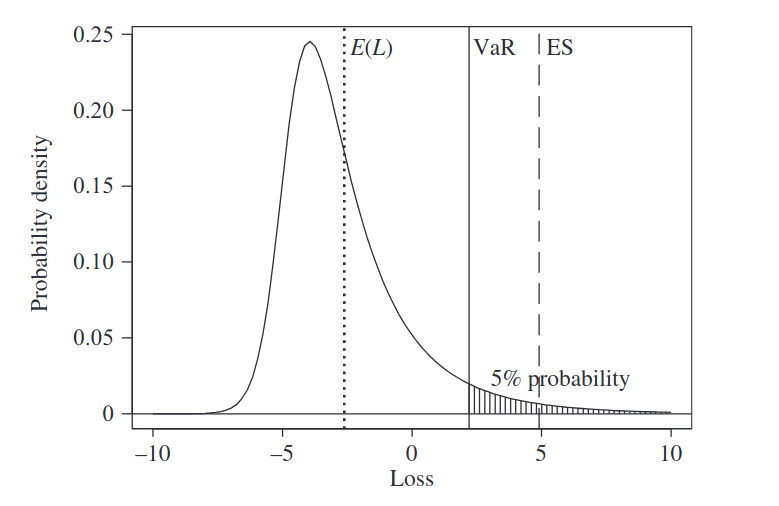
\includegraphics[width=\linewidth]{../img/VaR_CVaR_graph_theory.png}
  \caption{Illustration of $VaR_{0.95}$ and $CVaR_{0.95}$ (where $CVaR_{0.95}$ is labeled as ES). Image sourced from \cite[Figure 2.2.]{mcneil2015quantitative}. \textcolor{red}{TODO: generate the figure myself}}
  \label{fig:VaR_CVaR_graph_theory}
\end{figure}


Value at risk also comes with several advantages and disadvantages. While it is simple to understand and globally accepted by regulators, it is not coherent in general (the subadditivity requirement is not fulfilled), it doesn't quantify the losses exceeding $VaR_{\alpha}(x)$ and it is not convex (this makes it hard to optimize a portfolio with regard to value at risk).

Due to the aforementioned disadvantages of value at risk, another risk measure was considered.
Considering the expected loss exceeding the $VaR_{\alpha}(x)$ level leads to the notion of \textit{Conditional value at risk}. \todo{Add conditional value at risk.}

\begin{defn}{Conditional value at risk} 
\label{cvar_definition}
\\  
\cite[p. 275]{cornuejols_tutuncu_2006}
\\
Let $\alpha$ be the chosen confidence level and let $\mathcal{L}(x,\Upsilon)$ have the meaning of loss distribution as defined above and assume that $\mathbb{E}(\abs{\mathcal{L}(x,\Upsilon)})<\infty$. Then the conditional value at risk or expected shortfall $CVaR_{\alpha}(x)$ is defined as
\begin{equation}
CVaR_{\alpha}(x)=\frac{1}{1-\alpha}\int_{f(x,y) \geq VaR_{\alpha}(x)} f(x,y)p(y) \, \mathrm{d} y.
\end{equation}
\end{defn}
Compared to value at risk, conditional value at risk is a coherent risk measure (for the proof, see \cite[Example 2.26.]{mcneil2015quantitative}), but since value at risk is present in its definition, optimizing a portfolio with regard to conditional value at risk according to this definition suffers from many of the same problems as optimizing a portfolio with regard to value at risk. Therefore, a new method has been developed in \cite{Rockafellar2000OptimizationOC} that allows optimization of conditional value at risk without computing value at risk using linear programming.

\section{Minimising CVaR using scenarios}
In this section, we closely follow the exposition provided in \cite[p. 275-278]{cornuejols_tutuncu_2006}.
Let
\begin{equation}
\label{eq:cvar_approx}
F_{\alpha}(x,\gamma)=\gamma + \frac{1}{1-\alpha} \int_{f(x,y) \geq \gamma} (f(x,y)-\gamma)p(y) \, \mathrm{d}y.
\end{equation}
The function $F_{\alpha}(x,\gamma)$ has three important properties:
\begin{lemma}{Properties of $F_{\alpha}(x,\gamma)$ \cite[p. 276]{cornuejols_tutuncu_2006}.}
\label{lemma:properties_of_cvar_approx} 
\\
The following three properties hold for $F_{\alpha}(x,\gamma)$:
\begin{enumerate}
	\item It is a convex function of $\gamma$.
	\item $VaR_{\alpha}(x)=\underset{\gamma}{\mathrm{argmin}} \, F_{\alpha}(x,\gamma)$.
	\item $ CVaR_{\alpha}(x) = \underset{\gamma}{\mathrm{min}} \, F_{\alpha}(x,\gamma)$.
\end{enumerate}
\end{lemma}
\begin{proof}
For the proof, see \cite[Theorems 1 and 2]{Rockafellar2000OptimizationOC}
\end{proof}
\subsection{CVaR formulation}
If we want to choose a portfolio $x$ that minimises $CVaR_{\alpha}(x)$, we can now do so by minimising $F_{\alpha}(x,\gamma)$ over $x \in \mathcal{X}$ and $\gamma \in \R$ (where $\mathcal{X}$ is some set of portfolios) thanks to the third property in Lemma \ref{lemma:properties_of_cvar_approx}. Of course, Equation \ref{eq:cvar_approx} is not particularly suitable for numerical computations. In practice, as was explained in detail in Chapter \ref{chap1}, the distribution of $\Upsilon$ is approximated using scenarios $\gamma_s$ with associated probabilities $p_s, s=1,\dots,S$.

We can then calculate an approximation of $F_{\alpha}(x,\gamma)$ as
\begin{equation}
\label{eq:cvar_approx_approx}
\hat{F}_{\alpha}(x,\gamma)=\gamma + \frac{1}{1-\alpha} \sum_{s=1}^S  p_s \max (f(x,\gamma_s)- \gamma,0).
\end{equation}
We have arrived at the optimization problem
\begin{equation}
\label{eq:cvar_optim_first}
\underset{x \in \mathcal{X}, \gamma}{\min} \hat{F}_{\alpha}(x,\gamma)= \underset{x \in \mathcal{X}, \gamma}{\min} \gamma + \frac{1}{1-\alpha} \sum_{s=1}^S p_s \max (f(x,\gamma_s)-\gamma,0).
\end{equation}
A trick can be used to turn Equation \ref{eq:cvar_optim_first} into a linear programming problem. If we create new variables $z_s \geq 0$ such that $z_s \geq f(x,\gamma_s)-\gamma$, we can write:
\begin{alignat}{10}
& \underset{x \in \mathcal{X}, z_s \geq 0, \gamma}{\min}  \, \, \, && \gamma + \frac{1}{1-\alpha} \sum_{s=1}^S p_s z_s \\
&s.t. && \, z_s \geq f(x,\gamma_s)-\gamma, s=1,\dots,S
\end{alignat}
which is a linear programming problem.
\subsection{Mean-CVaR formulation}
In this section, we present a more precise formulation for practical use adopted from \cite{cvar_robust_mean_cvar_portfolio_optimization}, particularly when we want to choose a portfolio that minimises the conditional value at risk and also allows for controlling the minimum expected return or setting the degree of risk aversion.
\subsubsection*{Formulation with minimum expected return}
Let $x=(x_1,\dots,x_n)$ be a vector denoting of weights of each of $n$ assets in a portfolio and consider that $\mu=(\mu_1,\dots,\mu_n)$ is a random vector representing the returns of the assets. Consider $S$ scenarios, each with probability $p_s$ and let $r_s = (r_{1,s},\dots,r_{n,s})$ be the particular realisation of $\mu$ in scenario $s$ and let $r_0$ be the minimum required expected return. For simplicity, we do not allow short selling (condition $x_i \geq 0, i=1,\dots,n$). Then we can write
\begin{alignat}{10}
& \underset{x_i \geq 0 , z_s \geq 0, \gamma}{\min}  \, \, \, && \gamma + \frac{1}{(1-\alpha)} \sum_{s=1}^S p_s z_s, \label{cvar_expected_return}  \\
&s.t. && \, z_s \geq  -\sum_{i=1}^{n} x_i r_{i,s} -\gamma, s=1,\dots,S, \nonumber \\
&  && \sum_{i=1}^{n} x_i \bar{R_i} \geq r_0, \label{eq:cvar_expected_return:min_return_equation} \\
&  && \sum_{i=1}^{n} x_i = 1, \nonumber
\end{alignat}
where $\bar{R_i}=\sum_{s=1}^{S}p_s r_{i,s}$, which is still a linear programming problem. Equation \ref{eq:cvar_expected_return:min_return_equation} assures the minimal expected return.
\subsubsection*{Formulation using risk aversion}
Another equivalent formulation might be useful when the decision maker does not require a minimum expected return explicitly, but rather wants to set his risk aversion expectations. This can be achieved by introducing a risk aversion parameter $\lambda \geq 0$ and writing
\begin{alignat}{10}
& \underset{x_i \geq 0 , z_s \geq 0, \gamma}{\min}  \, \, \, && \sum_{i=1}^{n} x_i \bar{R_i} + \lambda \left( \gamma + \frac{1}{(1-\alpha)} \sum_{s=1}^S p_s z_s \right), \label{eq:cvar_risk_aversion} \\
&s.t. && \, z_s \geq  -\sum_{i=1}^{n} x_i r_{i,s} -\gamma, s=1,\dots,S, \nonumber \\
&  && \sum_{i=1}^{n} x_i = 1. \nonumber
\end{alignat}
\section{Minimising CVaR using scenarios in multistage setting}
In the multistage setting, the problem is a bit more complicated. Since the returns now do not occur at one single time but rather it is a sequence of returns, the notion of a risk measure must be extended accordingly. For the purposes of this thesis, we focus on the \textit{end of horizon $CVaR$}, for more advanced topics such as \textit{Nested $CVaR$ model} or \textit{Sum of $CVaR$ model}, we refer the reader to the summary in \cite[Section 1.4.]{kozmikv_phdthesis}.

\subsection{End of horizon CVaR}

\begin{defn}{End of horizon $CVaR$.} \\
Consider Definition \ref{cvar_definition}. If we consider the $CVaR$ calculated from the last stage (at the end of the investment horizon), we call it end of horizon $CVaR$.
\end{defn}
The definition of \textit{end of horizon $CVaR$} is very similar to the definition of regular $CVaR$, with the small difference that the multistage formulation now allows the decision maker to reallocate funds during the investment period (at the end of each stage). 

\subsubsection{End of horizon CVaR - scenario formulation}
We now extend Formulations \ref{cvar_expected_return} and \ref{eq:cvar_risk_aversion} to the multistage case. Consider we want to optimise a portfolio consisting of $n$ stocks over $T$ stages and consider a scenario tree with $S$ leaves (here we abuse notation and write sets $S=\{1,\dots,S\}$, $T=\{1,\dots,T\}$ and $I=\{1,\dots,n\})$. The problem \ref{cvar_expected_return} can then be reformulated as Equation \ref{eq:cvar_multistage_expected_return} by introducing variables $w_{t,s}$ which represent the wealth in scenario $s$ at time $t$ and $tot_s$ which is the total return in scenario $s$.

\begin{alignat}{10}
& \min \, \, \, && \gamma + \frac{1}{(1-\alpha)} \sum_{s=1}^S p_s z_s, \label{eq:cvar_multistage_expected_return}  \\
&s.t. && \, z_s \geq  -tot_s -\gamma, \forall s \in S \nonumber \\
&  && \sum_{s=1}^{S} p_s tot_s \geq r_0, \nonumber \\
& && w_{1,s}=1, \forall s \in S, \nonumber \\
& && w_{t,s}=\sum_{i=1}^{n} x_{i,t,s}, \forall s \in S, \forall t \in \{1,\dots,T-1\}, \label{eq:cvar_multistage_expected_return:wealth_distribution} \\
& && w_{t+1,s}=\sum_{i=1}^{n} r_{i,t,s} x_{i,t,s}, \forall s \in S, \forall t \in \{1,\dots ,T-1\}, \label{eq:cvar_multistage_expected_return:wealth_increases} \\
& && tot_s = \frac{w_{T,s}}{w_{1,s}}, \forall s \in S, \nonumber \\
& && z_s \geq 0, \forall s \in S, \nonumber \\
& && x_{i,t,s} \geq 0, \forall s \in S, \forall i \in I, \forall t \in \{1,\dots ,T-1\}, \nonumber \\
& && \gamma \in \R ,\nonumber \\
& && + \mathrm{nonanticipativity \, constraints}, \nonumber
\end{alignat}
The initial wealth $w_{1,s}$ is set to 1 and in each stage, the wealth increases by the returns obtained in the previous stage (Equation \ref{eq:cvar_multistage_expected_return:wealth_increases}) and is distributed again (Equation \ref{eq:cvar_multistage_expected_return:wealth_distribution}, at the end of the investment horizon we do not need to distribute the wealth into assets again). $r_{i,t,s}$ is the return obtained from stock $i$ at stage $t$ in scenario $s$ (we consider returns indexed by $t$ to occur at the end of stage $t$ (after the portfolio allocations $x_{i,t,s}$ are set), so that Equation \ref{eq:cvar_multistage_expected_return:wealth_increases} makes sense). The returns $r_{i,t,s}$ are of the form $1+r$ (where if the asset gained 6 percent, then $r_{i,t,s}=1.06$). This justifies Equation \ref{eq:cvar_multistage_expected_return:wealth_increases}. $tot_s \, \forall s \in S$ and $r_0$ are then again of the form $1+r$.

\begin{rem}
We do not include the nonanticipativity constraints in the above formulation, since they must be specified explicitly according to the structure of the scenario tree. To illustrate the explicit formulation of nonanticipativity constraints, consider Figure \ref{fig:balanced_scenario_tree}. In the context of the above problem, there are 6 scenarios ($111, 112, 113, 121, 122, 123$). For this illustration, let $\mathbf{x}_{t,s}$ be the vector of allocations to each assets at time $t$ and in scenario $s$. The nonanticipativity constraints now read:
\begin{alignat}{10}
& && \mathbf{x}_{t1,111}=\mathbf{x}_{t1,112}=\mathbf{x}_{t1,113}=\mathbf{x}_{t1,121}=\mathbf{x}_{t1,122}=\mathbf{x}_{t1,123} \nonumber \\
& && \mathbf{x}_{t2,111}=\mathbf{x}_{t2,112}=\mathbf{x}_{t2,113},\mathbf{x}_{t2,121}=\mathbf{x}_{t2,122}=\mathbf{x}_{t2,123}. \nonumber
\end{alignat}
\end{rem}
Similarly, the problem \ref{eq:cvar_risk_aversion} can then be reformulated as Equation \ref{eq:cvar_multistage_risk_aversion}:

\begin{alignat}{10}
& \min  \, \, \, &&\sum_{s=1}^{S} p_s tot_s + \lambda \left( \gamma + \frac{1}{(1-\alpha)} \sum_{s=1}^S p_s z_s \right), \label{eq:cvar_multistage_risk_aversion}  \\
&s.t. && \, z_s \geq  -tot_s -\gamma, \forall s \in S \nonumber \\
& && w_{1,s}=1, \forall s \in S, \nonumber \\
& && w_{t,s}=\sum_{i=1}^{n} x_{i,t,s}, \forall s \in S, \forall t \in \{1,\dots ,T-1\}, \label{eq:cvar_multistage_expected_return:wealth_distribution_risk_aversion} \\
& && w_{t+1,s}=\sum_{i=1}^{n} r_{i,t,s} x_{i,t,s}, \forall s \in S, \forall t \in \{1,\dots ,T-1\}, \label{eq:cvar_multistage_expected_return:wealth_increases_risk_aversion} \\
& && tot_s = \frac{w_{T,s}}{w_{1,s}}, \forall s \in S, \nonumber \\
& && z_s \geq 0, \forall s \in S, \nonumber \\
& && x_{i,t,s} \geq 0, \forall s \in S, \forall i \in I, \forall t \in \{1,\dots ,T-1\}, \nonumber \\
& && \gamma \in \R ,\nonumber \\
& && + \mathrm{nonanticipativity \, constraints}, \nonumber
\end{alignat}
where $\lambda \geq 0$ is a risk aversion parameter and the nonanticipativity constraints would again need to be provided explicitly according to the structure of the scenario tree.